\documentclass[12pt,a4paper]{article}
\usepackage{physics}
\usepackage{amssymb, amsmath}
\usepackage{subcaption}
\newcommand{\activity}{Activity 16 -- Support Vector Machines}
\input{spp.dat}

\begin{document}

\title{\TitleFont \activity}
\author[ ]{\textbf{Kenneth V. Domingo} \\
2015--03116 \\
App Physics 186, 1\textsuperscript{st} Semester, A.Y. 2019--20}
\affil[ ]{\corremail{kvdomingo@up.edu.ph} }

\maketitle
\thispagestyle{titlestyle}

\section*{Results and Discussion}
\setcounter{section}{1}

For this activity \cite{soriano,veksler}, I used the extracted fruit color features in $a^*-b^*$ space from a previous activity. I used only the data for oranges and apples, and assigned them labels of $-1$ \& $+1$, respectively. The objective for SVM is

\begin{equation} \label{eq:objective}
	\min \frac{1}{2} \norm{\vec{w}}_2^2 \quad \textrm{subject to} \quad y_i \qty(\vec{w}^\top \vec{x}_i + b) \geq 1 \quad \forall i
\end{equation}

\noindent which is a quadratic and hence, convex problem. Here, $\vec{w}$ is the reference vector perpendicular to the decision line, $\vec{x}$ is the feature vector, $y$ is the output classification, and $b$ is the bias. Using the Python \texttt{CVXPY} library \cite{cvxpy}, we can setup the above objective and constraint as-is and directly obtain $\vec{w}$. Since we have two features, the separating hyperplane is a line defined by

\begin{equation}
	g(x) = -\frac{w_1}{w_2}x - \frac{b}{w_2}
\end{equation}

\noindent where $w_i$ are the elements of $\vec{w}$. The width of the margin is defined by

\begin{equation}
	m = \frac{1}{\norm{\vec{w}}_2}
\end{equation}

\noindent so we can plot the margins on opposite sides of the decision line using trigonometric identities:

\begin{equation}
	g_\pm(x) = g(x) \pm m \sqrt{1 + \qty(\frac{w_1}{w_2})^2}
\end{equation}

\noindent Figure \ref{fig:svm-db} shows the optimum decision boundary with maximized margins in the $a^*-b^*$ feature space, along with the input data points and support vectors.

\begin{figure}[htb]
	\centering
	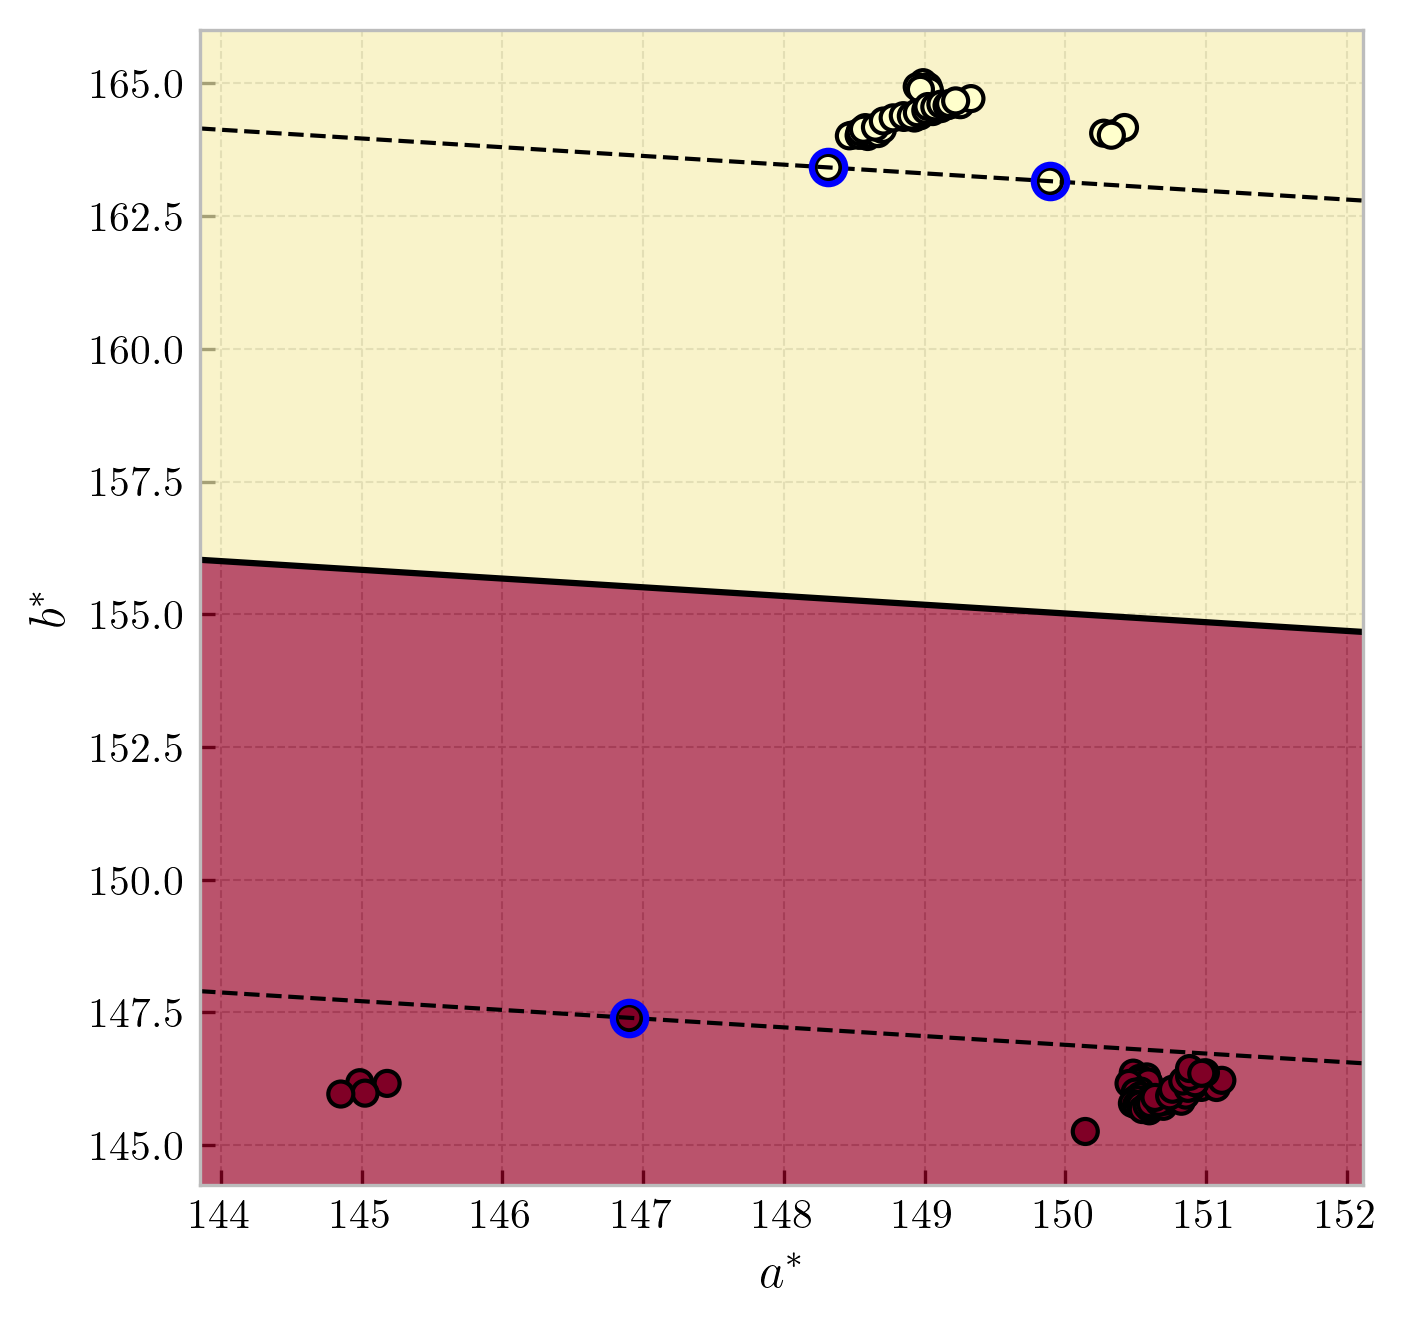
\includegraphics[width=0.75\textwidth]{svm-db.png}
	\caption{Decision boundary for oranges and apples data in $a^*-b^*$ feature space. The yellow region corresponds to a classification of $-1$ (oranges), while the red region corresponds to $+1$ (apples). The vectors highlighted in blue are the support vectors. The solid line is the decision boundary, while the dashed lines are the margins.}
	\label{fig:svm-db}
\end{figure}

\clearpage
\begin{table}[!htb]
	\centering
	\caption{Self-evaluation.}
	\begin{tabular}{||r|c||}
		\hline
		Technical correctness & 5 \\ \hline
		Quality of presentation & 5 \\ \hline
		Initiative & 0 \\ \hline
		\textbf{TOTAL} & \textbf{10} \\ \hline
	\end{tabular}
	\label{tab:self-eval}
\end{table}

\bibliographystyle{spp-bst}
\bibliography{biblio}

\end{document}